%%%%%%%%%%%%%%%%%%%%%%%%%%%%%%%%%%%%%%%%%
% Compact Academic CV
% LaTeX Template
% Version 2.0 (6/7/2019)
%
% This template originates from:
% https://www.LaTeXTemplates.com
%
% Authors:
% Dario Taraborelli (http://nitens.org/taraborelli/home)
% Vel (vel@LaTeXTemplates.com) 
%
% License:
% CC BY-NC-SA 3.0 (http://creativecommons.org/licenses/by-nc-sa/3.0/)
%
%%%%%%%%%%%%%%%%%%%%%%%%%%%%%%%%%%%%%%%%%

%----------------------------------------------------------------------------------------
%	PACKAGES AND OTHER DOCUMENT CONFIGURATIONS
%----------------------------------------------------------------------------------------

\documentclass[11pt]{article} % Default document font size

%%%%%%%%%%%%%%%%%%%%%%%%%%%%%%%%%%%%%%%%%
% Compact Academic CV
% Structural Definitions
% Version 1.0 (6/7/2019)
%
% This template originates from:
% https://www.LaTeXTemplates.com
%
% Authors:
% Dario Taraborelli (http://nitens.org/taraborelli/home)
% Vel (vel@LaTeXTemplates.com)
%
% License:
% CC BY-NC-SA 3.0 (http://creativecommons.org/licenses/by-nc-sa/3.0/)
%
%%%%%%%%%%%%%%%%%%%%%%%%%%%%%%%%%%%%%%%%%

%----------------------------------------------------------------------------------------
%	REQUIRED PACKAGES AND MISC CONFIGURATIONS
%----------------------------------------------------------------------------------------

\usepackage{graphicx} % Required for including images

\setlength{\parindent}{0pt} % Stop paragraph indentation

%----------------------------------------------------------------------------------------
%	MARGINS
%----------------------------------------------------------------------------------------

\usepackage{geometry} % Required for adjusting page dimensions and margins

\geometry{
	paper=a4paper, % Paper size, change to letterpaper for US letter size
	top=3.25cm, % Top margin
	bottom=4cm, % Bottom margin
	left=3.5cm, % Left margin
	right=3.5cm, % Right margin
	headheight=0.75cm, % Header height
	footskip=1cm, % Space from the bottom margin to the baseline of the footer
	headsep=0.75cm, % Space from the top margin to the baseline of the header
	%showframe, % Uncomment to show how the type block is set on the page
}

%----------------------------------------------------------------------------------------
%	FONTS
%----------------------------------------------------------------------------------------

\usepackage[utf8]{inputenc} % Required for inputting international characters
\usepackage[T1]{fontenc} % Output font encoding for international characters

%\usepackage[semibold]{ebgaramond} % Use the EB Garamond font with a reduced bold weight

%----------------------------------------------------------------------------------------
%	SECTION STYLING
%----------------------------------------------------------------------------------------

%\usepackage{sectsty} % Allows changing the font options for sections in a document

%\sectionfont{\fontsize{13.5pt}{18pt}\selectfont} % Set font options for sections
%\subsectionfont{\mdseries\scshape\normalsize} % Set font options for subsections
%\subsubsectionfont{\mdseries\upshape\bfseries\normalsize} % Set font options for subsubsections

%----------------------------------------------------------------------------------------
%	MARGIN YEARS
%----------------------------------------------------------------------------------------

\usepackage{marginnote} % Required to output text in the margin

\newcommand{\years}[1]{\marginnote{\scriptsize #1}} % New command for adding years to the margin
\renewcommand*{\raggedleftmarginnote}{} % Left-align the years in the margin
\setlength{\marginparsep}{-10pt} % Move the margin content closer to the text
\reversemarginpar % Margin text to be output into the left margin instead of the default right margin

%----------------------------------------------------------------------------------------
%	COLOURS
%----------------------------------------------------------------------------------------

\usepackage[usenames, dvipsnames]{xcolor} % Required for specifying colours by name

%----------------------------------------------------------------------------------------
%	LINKS
%----------------------------------------------------------------------------------------

\usepackage[bookmarks, colorlinks, breaklinks]{hyperref} % Required for links

% Set link colours
\hypersetup{
	linkcolor=blue,
	citecolor=blue,
	filecolor=black,
	urlcolor=MidnightBlue
}

\renewcommand\labelenumi{[\theenumi]}
 % Include the file specifying the document structure and styling

% Set PDF meta-information
\hypersetup{
	pdftitle={Yunlei Wang - Curriculum vitae},
	pdfauthor={Yunlei Wang}
}

%----------------------------------------------------------------------------------------
\begin{document}

%----------------------------------------------------------------------------------------
%	CONTACT AND GENERAL INFORMATION
%----------------------------------------------------------------------------------------

\begin{center}
{\huge \bfseries\scshape Curriculum Vitae}
\end{center}
\vspace{0.05\textheight}
{\LARGE\bfseries Yunlei Wang}% Name
\bigskip % Whitespace

China University of Geosciences Wuhan (CUG)\\ % Address
Office 1101\\ New Office Building of CUG
%\medskip % Whitespace

\vspace{0.01\textheight} 

Mobile: +86 13936256225\\ % Mobile number
Email: \href{wcghdpwyl@gmail.com}{wcghdpwyl@gmail.com}\\% Email address
% Webpage: \href{http://rieunity.github.io}{http://rieunity.github.io}% Academic/personal website
\vspace{0.01\textheight}% Whitespace between contact information and specific CV information
%------------------------------------------------
Date of birth: April 23, 1993\\
Gender: Male\\
Birth place:Lu'an, Anhui province, China\\ % Date of birth
Nationality: China\hfill \smash{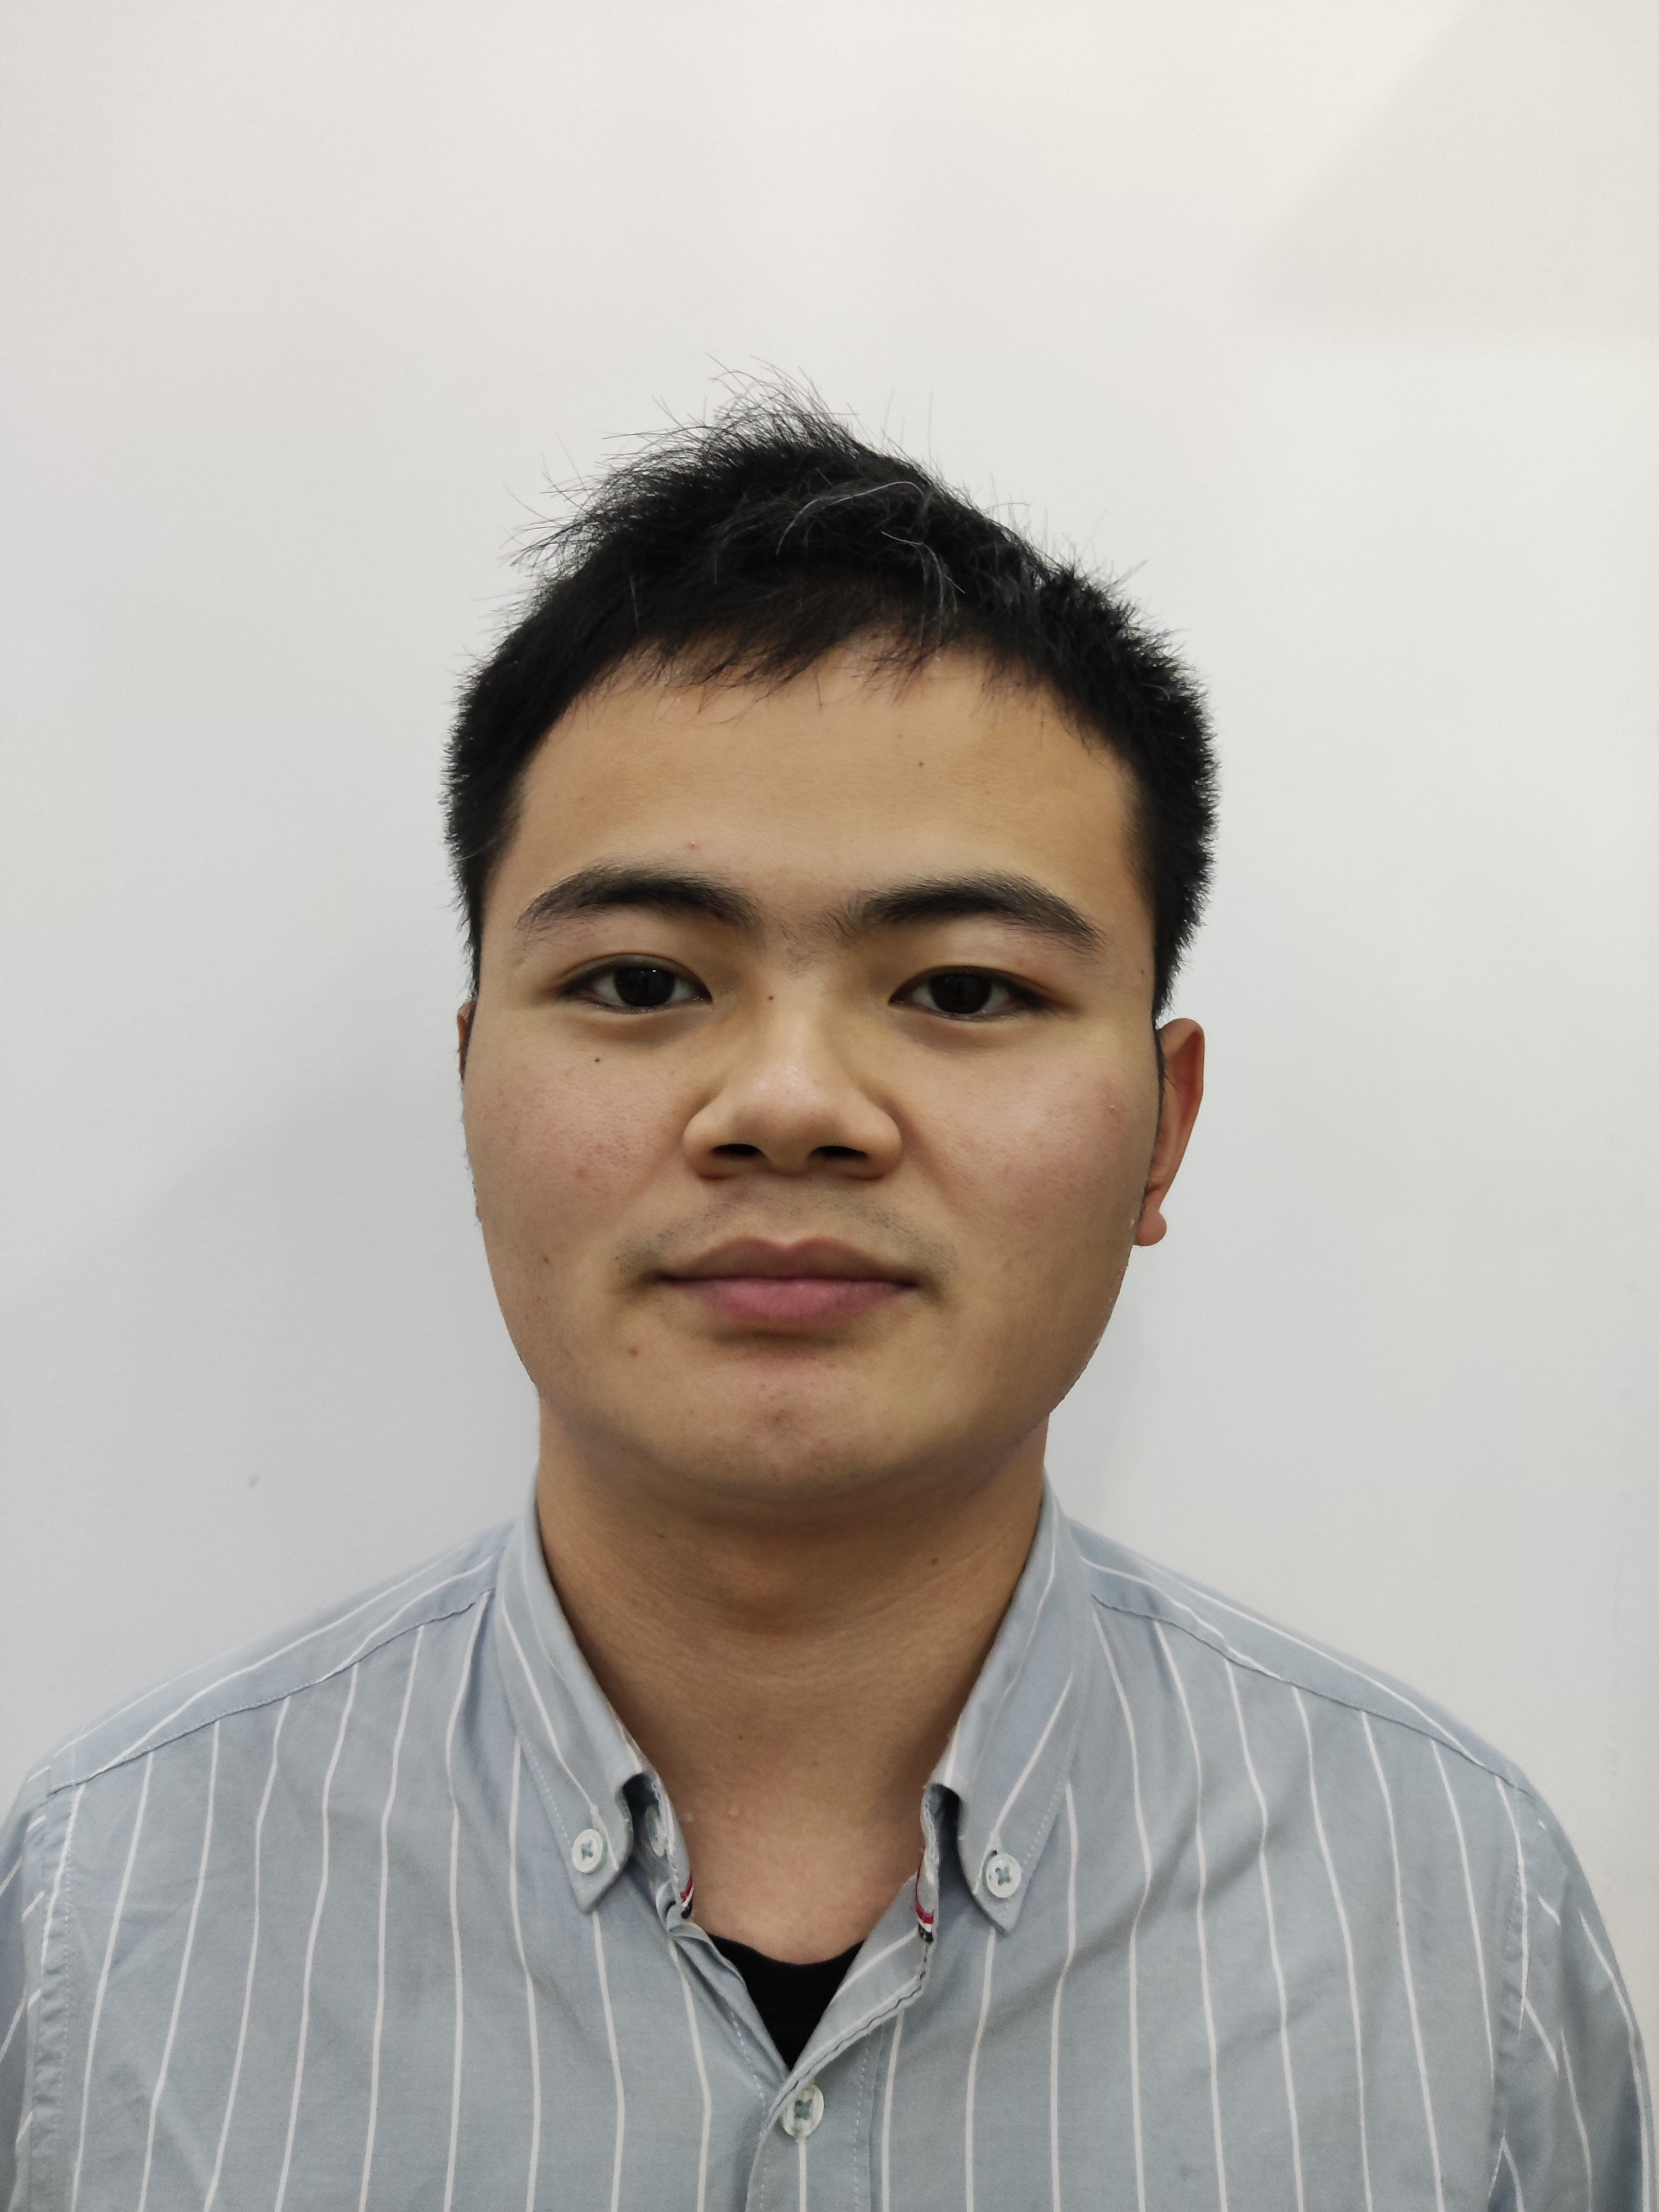
\includegraphics[width=4.25cm]{me}} % Nationality

%----------------------------------------------------------------------------------------
%	EDUCATION
%----------------------------------------------------------------------------------------

\section*{Education}

\years{2019-}\textsc{MSc} in Mathematics, School of Mathematics and Physics, China University of Geosciences (Wuhan), expected by July 2022\\
advisor: Prof. Ming Wang\\
GPA: 3.87/4 \\
\years{2015, fall} Exchange students in Department of Physics,  Fudan University\\
\years{2012-2016}\textsc{BSc} in Applied Physics, School of Science, Harbin Institute of Technology \\
GPA: 3.74/4 

%----------------------------------------------------------------------------------------
%	GRANTS, HONOURS AND AWARDS
%----------------------------------------------------------------------------------------

\section*{Research interests \& experiences}
My interests lie in harmonic analysis and partial differential equations.

Now I am focusing on uncertainty principles in harmonic analysis, especially its applications in quantitative unique continuation and control of PDEs. 

\section*{Activities \& competitions}
\years{2015.7} Summer Camp of Theoretical Physics, Peiking University\\
\years{2014.3} The Chinese Mathematics Competitions, the third prize  in the final\\
\years{2012.7} Physics Enlightment Summer School of National Top Students, Nanjing University

%\section*{Conference attended}

\section*{Teaching assistance}
2019 Fall, Real Analysis, China University of Geosciences (Wuhan) \\
2020 Spring, Functional Analysis, China University of Geosciences (Wuhan)
%----------------------------------------------------------------------------------------
%	PUBLICATIONS AND TALKS
%----------------------------------------------------------------------------------------


\section*{Publications}
\begin{enumerate}
\leftskip-0.13in
\item Yunlei Wang, Ming Wang, Observability inequality at two time points for the KdV equation from measurable sets, \emph{J. Math. Anal. Appl.} 505 (2022), no. 2, Paper No. 125643, 15pp.
\end{enumerate}
\iffalse
\subsection*{Journal articles}


\years{1905a}Einstein, Albert (1905), “On a Heuristic Viewpoint Concerning the Production and Transformation of Light", \emph{Annalen der Physik} 17: 132–148.\\
\years{1905b}Einstein, Albert (1905), A new determination of molecular dimensions. \emph{PhD dissertation}.\\
\years{1905c}Einstein, Albert (1905), “On the Motion—Required by the Molecular Kinetic Theory of Heat—of Small Particles Suspended in a Stationary Liquid", \emph{Annalen der Physik} 17: 549–560.\\
\years{1905d}Einstein, Albert (1905), “On the Electrodynamics of Moving Bodies", \emph{Annalen der Physik} 17: 891–921.\\
\years{1905e}Einstein, Albert (1905), “Does the Inertia of a Body Depend Upon Its Energy Content?", \emph{Annalen der Physik} 18: 639–641.\\
\years{1915}Einstein, Albert (1915), “Die Feldgleichungen der Gravitation (The Field Equations of Gravitation)", \emph{Koniglich Preussische Akademie der Wissenschaften}: 844–847\\
\years{1917a}Einstein, Albert (1917), “Kosmologische Betrachtungen zur allgemeinen Relativitätstheorie (Cosmological Considerations in the General Theory of Relativity)", \emph{Koniglich Preussische Akademie der Wissenschaften}\\
\years{1917b}Einstein, Albert (1917), “Zur Quantentheorie der Strahlung (On the Quantum Mechanics of Radiation)", \emph{Physikalische Zeitschrift} 18: 121–128

%------------------------------------------------

\subsection*{Books}

\years{1954}Einstein, Albert (1954), \emph{Ideas and Opinions}, New York: Random House, ISBN 0-517-00393-7

%------------------------------------------------

\subsection*{Newspaper articles}

\years{1940}Einstein, Albert, et al. (December 4, 1948), “To the editors", \emph{New York Times}\\
\years{1949}Einstein, Albert (May 1949), “Why Socialism?", \emph{Monthly Review}.

%----------------------------------------------------------------------------------------
%	TEACHING
%----------------------------------------------------------------------------------------

\section*{Teaching}

\ldots

%------------------------------------------------

\section*{Service to the profession}

\ldots

\vfill % Whitespace before final footer

%----------------------------------------------------------------------------------------
%	FINAL FOOTER
%----------------------------------------------------------------------------------------

% Any final footer text such as a URL to the latest version of this CV, last updated date, compiled in XeTeX, etc
\fi
\begin{center}
	\scriptsize
	Last updated: \today
\end{center}

%----------------------------------------------------------------------------------------

\end{document}
